%----------------------------------------
% SECTION: Toric Code and its features
%----------------------------------------
\section{Toric Code and its features}
\label{sec:toric_code_and_its_features}

The Toric code is two-dimensional model of spin-\onehalf degrees of freedom (d.o.f), which can be regarded as an example of a pure $\mathbb{Z}_2$ lattice gauge theory.
In particular, we focus on a $L \times L$ square lattice with periodic boundary conditions.
The \dof are defined on the links the lattice, where the local Hilbert space is $\C^2$.
The main operators we are going to use are the Pauli matrices
\begin{equation}
    X = \begin{pmatrix}
        0 & 1 \\ 1 & 0
    \end{pmatrix}
    \qand
    Z = \begin{pmatrix}
        1 & 0 \\ 0 & -1
    \end{pmatrix},
    \label{eq:matrices_X_Z}
\end{equation}
which we have written in the computational basis $\{\ket{0}, \ket{1}\}$, where the $Z$-matrix is diagonal.
It is important to remember that the matrices $X$ and $Z$ \emph{anticommutes}.
\begin{equation}
    [X, Z] = 0.
\end{equation}

The main \emph{local} operators that enters the Hamiltonian are defined on the \emph{stars} and \emph{plaquettes} of the lattice.
The term \emph{star} refers to the links attached to a common vertex $v$, while by \emph{plaquette} $p$ we mean the links around a face of the lattice.
A \emph{star operator} and a \emph{plaquette operator} are respectively defined as
\begin{equation}
    A_v = \prod_{\link \in s} Z_\link, \qquad
    B_p = \prod_{\link \in p} X_\link.
    \label{eq:star_plaq_op_def}
\end{equation}
where $v$ is a vertex and $p$ a plaquette (see Fig.~\ref{fig:toric_code_operators}).
One can easily see that
\begin{equation}
    \comm{A_v}{A_{v^{\prime}}} = 0 \qand
    \comm{B_p}{B_{p^{\prime}}} = 0
    \label{eq:star_plaq_op_comm_1}
\end{equation}
for all vertices $v$ and $v^{\prime} $, and all plaquettes $p$ and $p^{\prime} $.
But it is also true that
\begin{equation}
    \comm{A_v}{B_p} = 0
    \label{eq:star_plaq_op_comm_2}
\end{equation}
for all $v$ and $p$.
This is because a star and a plaquette share zero or two links, so the signs factors from the anticommutation of $X$ and $Z$ cancel out.
The eigenvalues of the Pauli matrices are just $\pm 1$, so the same holds true for $A_s$ and $B_p$.
Moreover, like the Pauli matrices, also $A_s^2 = \identity$ and $B_p^2 = \identity$.


Now, given the operators in \eqref{eq:star_plaq_op_def}, we can write down the Hamiltonian of the Toric Code:
\begin{equation}
    H = - \sum_{v} A_v - \sum_{p} B_p
    \label{eq:toric_code_hamiltonian}
\end{equation}
which is \emph{exactly solvable}, due to \eqref{eq:star_plaq_op_comm_1} and \eqref{eq:star_plaq_op_comm_2}.
\begin{figure}[t]
    \centering
    \begin{tikzpicture}[
        scale=1.2,
        site/.style = {circle, inner sep=0 pt, minimum size=3pt, draw=black, fill=white},
        plaq/.style={blue, ultra thick},
        gauss/.style={red, ultra thick}
        ]
    % Lattice
    \draw[thin] (-0.5,-0.5) grid (4.5,2.5);

    % Plaquette operator
    \draw[plaq] (3,1) -- (4,1) node [pos=0.5, below] {$X$};
    \draw[plaq] (4,1) -- (4,2) node [pos=0.5, right] {$X$};
    \draw[plaq] (4,2) -- (3,2) node [pos=0.5, above] {$X$};
    \draw[plaq] (3,2) -- (3,1) node [pos=0.5, left]  {$X$};
    \draw[blue, ultra thick, pattern=north east lines, pattern color=blue] (3,1) rectangle (4,2);
    \draw (3.5,1.5) node [fill=white, rounded corners] {$B_p$};

    % Gauss operator
    \draw[gauss] (1, 1) -- (2, 1) node [pos=0.5, below right] {$Z$};
    \draw[gauss] (1, 1) -- (1, 2) node [pos=0.5, above left] {$Z$};
    \draw[gauss] (1, 1) -- (0, 1) node [pos=0.5, below left] {$Z$};
    \draw[gauss] (1, 1) -- (1, 0) node [pos=0.5, below right] {$Z$};

    \foreach \y in {0,1,2} \foreach \x in {0,1,...,4} \draw (\x,\y) node [site] {};

    \draw (1,1) node [above right, outer sep=5pt, inner sep=3pt, draw=red, rounded corners=3pt] {$A_s$};
\end{tikzpicture}

    \caption{Graphical representation of the Toric Code operators $A_s$ and $B_p$}
    \label{fig:toric_code_operators}
\end{figure}



%
% SUBSECTION: Topological ground states
%
\subsection{Topological Ground states}
\label{sub:topological_ground_states}

Given the commutation relations of the $A_v$ and $B_p$ operators in \eqref{eq:star_plaq_op_comm_1} and \eqref{eq:star_plaq_op_comm_2}, one can find the ground state $\ket{\Omega}$ by simply imposing the constraints
\begin{equation}
    A_v \ket{\Omega} = \ket{\Omega} \qand
    B_p \ket{\Omega} = \ket{\Omega}, \qquad \forall v,\, p.
    \label{eq:ground_state_constraints}
\end{equation}
From these constraints one can explicitly construct a ground state for the Toric Code in the following way.
Working in the $Z$-basis, we can start from
\begin{equation}
    \ket{0}_{\text{TC}} = \bigotimes_{\link \in \lattice} \ket{0}_{\link},
\end{equation}
which is the state where every link is in the $\ket{0}$, where $Z \ket{0} = \ket{0}$.
This state obviously satisfy the first condition in \eqref{eq:ground_state_constraints}.

Now, regarding the $B_p$'s operators, consider a single plaquette in the state $\ket{0}_p$ where every link is in the $\ket{0}$ state.
The action of $B_p$ flips the state of every link, from $\ket{0}$ to $\ket{1}$, obtaining $\ket{1}_p$.
Therefore, a plaquette is in an eigenstate of $B_p$ if is in an equal superposition of $\ket{0}_p$ and $\ket{1}_p$.
Knowing this, it is straightforward to see that the operator $(\identity + B_p)/\sqrt{2}$ generates an eigenstate of $B_p$ from $\ket{0}_p$.
In fact, a simple calculation
\begin{equation}
    B_p \frac{\identity + B_p}{\sqrt{2}} \ket{0}_p = \frac{B_p + \identity}{\sqrt{2}} \ket{0}_p
\end{equation}
shows that we obtain an eigenstate of $B_p$ with eigenvalue $+1$, due to $B_p^2 = \identity$.

Therefore, we can obtain a ground state for the Toric code as
\begin{equation}
    \ket{\Omega} = \prod_{p} \frac{\identity + B_p}{\sqrt{2}} \ket{0}_{\text{TC}}.
\end{equation}
More generally, we can define the space of ground states
\begin{equation}
    \mathcal{G} = \qty{ \ket{\Omega} : A_s \ket{\Omega} = \ket{\Omega}, \quad B_p \ket{\Omega} = \ket{\Omega} \quad \forall s, p },
    \label{eq:TC_protected_subspace}
\end{equation}
which contents \emph{depends on the topology of the lattice}.
For example, later we will show that with \emph{periodic boundary conditions} then there are
\emph{four degenerate ground states}.


Consider a lattice $\lattice$ of size $L \times L$ with periodic boundary conditions in both directions, i.e.~a torus.
From \eqref{eq:ground_state_constraints}, we have $2L^2$ constraints.
These are not all independent because if we multiply them all, we obtain
\begin{equation}
    \prod_{v} A_v = \identity \qand
    \prod_{p} B_p = \identity,
\end{equation}
which actually means that there are $2L^2 - 2$ independent conditions.
The total Hilbert space has dimension $2^{2L^2}$.
Combined with $2L^2 - 2$ independent conditions we obtain $2^{2L^2 - 2L^2 + 2} = 4$ independent states.
Therefore, $\dim \mathcal{G} = 4$ because we have four degenerate distinct ground states.
These are eigenstates of all $A_v$ and $B_p$, with all the same eigenvalues.
Any other that commutes with the Hamiltonian is given by a product of $A_v$ and $B_p$, so it cannot distinguish the different ground states.


The only way to distinguish these ground states is through \emph{non-local operators} that commute with the Hamiltonian in \eqref{eq:toric_code_hamiltonian}.
Non-local in this instance means not expressible as a product or sum of vertex and plaquette operators.
But first let look more closely at \emph{local operators}.


Consider any region $\mathcal{R}$ on the lattice $\lattice$.
Without loss of generality, let $\mathcal{R}$ be a connected region, which means it is just a set of jointed plaquettes.
On this region $\mathcal{R}$ we can define a local operator $W$ as a product of $B_p$ operators:
\begin{equation}
    W = \prod_{p \in \mathcal{R}} B_p.
\end{equation}
This operator commutes will the terms of the Hamiltonian \eqref{eq:toric_code_hamiltonian}.
Due to $X^2 = \identity$, the previous equation can be rewritten as
\begin{equation}
    W = \prod_{\link \in \partial \mathcal{R}} X_{\link}.
\end{equation}
In other words, $W$ is equivalent to the product of $X$'s along the closed curve given by the boundary $\partial \mathcal{R}$ of $\mathcal{R}$.
In fact, the $B_p$ themselves are defined as product of $X$s along a closed curve, the plaquette.
In a sense, they are all \emph{string operators} on closed curves.

The same argument can be repeated for $A_v$ with the minor caveat that the dual lattice have to considered.
In the dual lattice $\duallattice$, to each plaquette $p$ of the lattice $\lattice$ corresponds a vertex $v$ on the dual lattice.
Then, to each link $\link$ in $\lattice$ corresponds a link $\link^{\ast}$ in $\duallattice$ in the perpendicular direction.
In this way, a star becomes a plaquette in the dual lattice.
From here, we can repeat the same argument.
Consider a region $\mathcal{R}^{\ast}$ a local operator $W^{\ast}$ such that
\begin{equation}
    W^{\ast} = \prod_{v \in \mathcal{R}^{\ast}} A_v,
\end{equation}
and, due to $Z^2 = \identity$, this is equal to
\begin{equation}
    W^{\ast} = \prod_{\link \in \partial \mathcal{R}^{\ast}} Z_{\link}.
\end{equation}
The local operator $W^{\ast}$ is a string of $Z$'s operators along the closed curve given by the boundary $\partial \mathcal{R}$ in $\duallattice$.
The same can be said for $A_v$, it is a string operator around the smallest possible curve in $\duallattice$.
% Indeed, a star on the direct lattice becomes a plaquette on the dual lattice.
% So a product of $A_v$ is equivalent to a string of $Z$ operators along closed curves on the dual lattice.
% All these curve have a common property, they are \emph{contractible}, meaning that they can be continuously deformed to a single point.
% The operators we have called local so far are string operators over contractible curves, but if we are on a lattice with non-trivial topology, like a torus, then we can also have \emph{non-contractible} curves.
We can conclude that all the local operators that commutes with Hamiltonian are just string operators over closed curve in either $\lattice$ or $\duallattice$.
But, these operators have alla a common feature, they are defined on \emph{contractible} curves.
Meaning that they can be ``continuously'' deformed to a single point.

\begin{figure}[t]
    \centering
    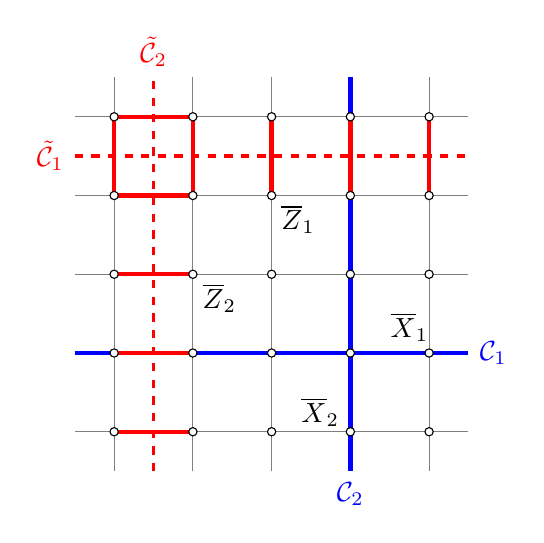
\begin{tikzpicture}[
        site/.style = {circle, inner sep=0 pt, minimum size=3pt, draw=black, fill=white},
    ]
    % lattice grid
    \draw[Gray,thin] (-0.5,-0.5) grid (4.5,4.5);

    % Wilson loops
    \draw[Blue, ultra thick]
        (-0.5, 1) -- (4.5, 1)
        node [pos=1, right] {$\mathcal{C}_1$}
        node [pos=0.85, above, black] {$\overline{X}_1$}
        ;
    \draw[Blue, ultra thick]
        (3, -0.5) -- (3, 4.5)
        node [pos=0, below] {$\mathcal{C}_2$}
        node [pos=0.15, left, black] {$\overline{X}_2$}
        ;

    % 't Hooft strings
    \draw[Red, very thick, dashed]
        (-0.5,3.5) -- (4.5,3.5)
        node[pos=0, left] {$\tilde{\mathcal{C}}_1$}
        ;
    \foreach \x in {0,...,4} { \draw[Red, ultra thick] (\x, 3) -- +(0, 1); }
    \draw (2,3) node [below right] {$\overline{Z}_1$};
    \draw[Red, very thick, dashed]
        (0.5,-0.5) -- (0.5,4.5)
        node[pos=1, above] {$\tilde{\mathcal{C}}_2$}
        ;
    \foreach \y in {0,...,4} { \draw[Red, ultra thick] (0, \y) -- +(1, 0); }
    \draw (1,2) node [below right] {$\overline{Z}_2$};
    \foreach \y in {0,...,4} \foreach \x in {0,...,4} \draw (\x,\y) node [site] {};
\end{tikzpicture}

    \caption{Non-contractible paths}
    \label{fig:nonlocal_operators_TC}
\end{figure}





String operators on non-contractible curves, either on the direct or dual lattice, are the non-local operators we have been looking for distinguish the states in $\mathcal{G}$.
Consider two non-contractible loops $\mathcal{L}_{1}$ and $\mathcal{L}_{2}$ on $\lattice$ along the $\hat{1}$ and $\hat{2}$ direction respectively, like in Fig.~\ref{fig:nonlocal_operators_TC}.
On these paths we can define the string operators $\overline{W}_1$ and $\overline{W}_2$ as
\begin{equation}
    \overline{W}_1 = \prod_{j \in \mathcal{C}_1}  \sigma^x_j, \qquad
    \overline{W}_2 = \prod_{j \in \mathcal{C}_2}  \sigma^x_j.
    \label{eq:nonlocal_X_operators}
\end{equation}
It can be proved that they commute with all the terms of the Hamiltonian, even though they cannot be expressed as a product of them.
The same can be repeated on the dual lattice $\duallattice$, by considering two non-contractible cuts $\mathcal{C}_1$ and $\mathcal{C}_2$ and defining $\overline{S}_1$ and $\overline{S}_2$ as
\begin{equation}
    \overline{S}_1 = \prod_{j \in \mathcal{C}_1}, \qquad
    \overline{S}_2 = \prod_{j \in \mathcal{C}_2}.
    \label{eq:nonlocal_Z_operators}
\end{equation}
Likewise, the operators in \eqref{eq:nonlocal_Z_operators} commutes with all the vertex and plaquettes operators but they do not commute with the operators in \eqref{eq:nonlocal_X_operators}.

In fact, \eqref{eq:nonlocal_X_operators} and \eqref{eq:nonlocal_Z_operators} anticommutes,
\begin{equation}
    \acomm*{\overline{W}_1}{\overline{S}_2} = 0 \qand
    \acomm*{\overline{W}_2}{\overline{S}_1} = 0,
\end{equation}
while
\begin{equation}
    \comm{\overline{W}_1}{\overline{W}_2} = 0 \qand
    \comm{\overline{S}_1}{\overline{S}_2} = 0.
\end{equation}
These relations can be thought as the same commutation relations of the $X$ and $Z$ gates of two qubits.

Therefore, the Toric Code (on a torus) has a protected subspace $\mathcal{G}$, see \eqref{eq:TC_protected_subspace}, that behaves like the Hilbert space of two qubits and the operators \eqref{eq:nonlocal_X_operators} and \eqref{eq:nonlocal_Z_operators} acts like unitary gates on this space.
Unfortunately, we cannot do quantum computation with these topological qubits because there is no entangling gates.
Nonetheless they can be used for storing information in a fault-tolerant way, because in order to flip a topological qubit you would need to act with a non-local operator that involves a large amount of links.


% \subsection{Particle excitations}%
% \label{sub:particle_excitations}
%
% Until now we have only discussed the ground states of the Toric Code, without touching the rest of the low energy sectors.
% In other words, how do we describe the excitations of this model?
% As we said, \eqref{eq:ground_state_constraints} are the set of constraints that defines the ground states.
% Therefore, every time a given state $\ket{\Psi}$ violates these equations, we will say that it contains \emph{particles}, which can be of different types.
% If $A_v \ket{\Psi} = - \ket{\Psi}$, then we will say that the vertex $v$ contains a $z$-type particle.
% Likewise, if $B_p \ket{\Psi} = - \ket{\Psi}$, then the plaquette $p$ contains a $x$-type particle.
%
% Now the question: starting from a ground state $\ket{\Omega}$, how can we introduce some particles?
% The answer is \emph{string operators}.
% We are not considering closed strings, like we did in Sec.~\ref{sub:topological_ground_states}, but any open string.
% The shortest open string that we can consider is a single link.
% So a $Z$-string on a single link is just $Z_j$, where $j$ is a label of a generic link.
% Consider now the state
% \begin{equation}
%     \ket*{\Psi^Z} = Z_j \ket{\Omega},
% \end{equation}
% This state hosts particles at the ``boundaries'' of the $j$-th link, i.e.~the vertices touching $j$ which we call $v_0$ and $v_1$.
% This can be proved by simply showing that $[ A_v, Z_j ] = 0$ for $v \neq v_0$ and $v \neq v_1$ and $\{ A_{v_0}, Z_j \} = \{ A_{v_1}, Z_j \} = 0$.
% Which immediately implies that
% \begin{equation}
%     A_{v_0} \ket*{\Psi^Z} = A_{v_1} \ket*{\Psi^Z} = - \ket*{\Psi^Z}
% \end{equation}
%


%
% SUBSECTION: Z2 Lattice gauge theory
%
\subsection{Toric Code as a \texorpdfstring{$\Z_2$}{Z2} Lattice Gauge Theory}
\label{sub:toric_code_as_a_z2_lattice_gauge_theory}

The Toric Code was formulated as a type of error-correcting code for quantum computing, but it can be reinterpreted as a pure $\Z_2$ lattice gauge theory.
This is a type of lattice gauge theory where we allow only two possible states for the gauge field.

On a single link, we consider the $X_{\link}$ as the gauge field operator, while $Z_{\link}$ the electric field operator.
In this way, we can automatically see that the term $B_p$ is the magnetic energy because it has the same form of single-plaquette Wilson loop.
Furthermore, the vertex operator $A_v$ can be read as a gauge transformation on the vertex $v$, because the $Z$'s operators flips the states in the $X$-basis, which would corresponds to gauge field configurations.

Now that we know the form of gauge transformations, we call a state \emph{physical} or \emph{gauge-invariant} if
\begin{equation}
    A_v \ket{\phi} = \ket{\phi} \quad \forall v \in \lattice,
    \label{eq:toric_code_physical_state}
\end{equation}
which leads to the definition of the \emph{physical Hilbert space}:
\begin{equation}
    \Hphys = \{\ket{\phi} \; \text{s.t.} \; A_v \ket{\phi} = \ket{\phi} \quad \forall v \in \lattice\}.
\end{equation}
For greater clarity, lets work in the \emph{electric basis}, which is just the $Z$-basis where the electric field is diagonal.
The electric field operator $Z$ has eigenvalue $+1$ and $-1$, corresponding respectively to the states $\ket{0}$ and $\ket{1}$.
In order to meet the condition in \eqref{eq:toric_code_physical_state}, a vertex configuration must have an even number of links in the $\ket{1}$ state (examples can be seen in Fig.~\ref{fig:gauge_inv_vertices_z2}).

\begin{figure}[t]
    \centering
    \begin{tikzpicture}[scale=0.35]

    % First row
    \draw[lattice] (-1.75, -1.75) grid (1.75, 1.75);
    \node[site] at (0, 0) {};

    \begin{scope}[xshift=4cm]
        \draw[lattice] (-1.75, -1.75) grid (1.75, 1.75);
        \draw[up] (-1.75, 0) -- (1.75, 0);
        \node[site] at (0, 0) {};
    \end{scope}

    \begin{scope}[xshift=8cm]
        \draw[lattice] (-1.75, -1.75) grid (1.75, 1.75);
        \draw[up] (0, -1.75) -- (0, 0) -- (1.75, 0);
        \node[site] at (0, 0) {};
    \end{scope}

    \begin{scope}[xshift=12cm]
        \draw[lattice] (-1.75, -1.75) grid (1.75, 1.75);
        \draw[up] (0, -1.75) -- (0, 0) -- (-1.75, 0);
        \node[site] at (0, 0) {};
    \end{scope}


    % Second row
    \begin{scope}[yshift=-4cm]
        \draw[lattice, up] (-1.75, -1.75) grid (1.75, 1.75);
        \node[site] at (0, 0) {};
    \end{scope}

    \begin{scope}[yshift=-4cm, xshift=4cm]
        \draw[lattice] (-1.75, -1.75) grid (1.75, 1.75);
        \draw[up] (0, -1.75) -- (0, 1.75);
        \node[site] at (0, 0) {};
    \end{scope}

    \begin{scope}[yshift=-4cm, xshift=8cm]
        \draw[lattice] (-1.75, -1.75) grid (1.75, 1.75);
        \draw[up] (0, 1.75) -- (0, 0) -- (1.75, 0);
        \node[site] at (0, 0) {};
    \end{scope}

    \begin{scope}[yshift=-4cm, xshift=12cm]
        \draw[lattice] (-1.75, -1.75) grid (1.75, 1.75);
        \draw[up] (-1.75, 0) -- (0, 0) -- (0, 1.75);
        \node[site] at (0, 0) {};
    \end{scope}


    % \node[font=\normalsize, right] at (14,0) {$\dots$};
\end{tikzpicture}

    \caption{Gauge invariant vertex states for the $\Z_2$ lattice gauge theory.}
    \label{fig:gauge_inv_vertices_z2}
\end{figure}

We have already argued that the $B_p$'s give the magnetic energy, and obviously the $Z$'s give the electric energy.
Hence, the pure gauge theory Hamiltonian is just
\begin{equation}
    H_{\Z_2} = - \sum_{p} B_p - \lambda \sum_{\link} Z_{\link},
    \label{eq:z2_lgt_hamiltonian}
\end{equation}
where $\lambda$ is a generic coupling that tunes the strength of the electric field with respect to the magnetic field.
Notice that we no longer have a dynamical vertex term in \eqref{eq:z2_lgt_hamiltonian} because we have imposed the condition \eqref{eq:toric_code_physical_state} on the physical states.

In order to better explain the different phases we can have by varying the coupling $\lambda$ in \eqref{eq:z2_lgt_hamiltonian}, we want to have a closer look at the physical states.
We have already seen that the condition \eqref{eq:toric_code_physical_state} constraints the types of vertex configurations.
From the allowed configuration, we can see that the only possible lattice states (in the electric basis) are states made of \emph{closed electric loops}.
An example of such state can be seen in Fig.~\ref{fig:physical_state_z2}.


\begin{figure}[t]
    \centering
    \begin{tikzpicture}[scale=0.5]
    \draw[lattice] (-1, -1) grid (11, 11);

    \draw[up] (0, 0) rectangle (2, 2);
    \draw[up] (6, 0) rectangle (10, 2);
    \draw[xshift=-2cm, up] (4, 4) -- (4, 10) -- (8, 10) -- (8, 6) -- (6, 6) -- (6, 4) -- cycle;
    \draw[up] (-1, 6) -- (0, 6) -- (0, 11);
    \draw[up] (11, 4) -- (8, 4) -- (8, 8) -- (11, 8);

    % sites
    \DrawSites{0,2,...,10}{0,2,...,10}
\end{tikzpicture}

    \caption{Example of a physical state in the $\Z_2$ lattice gauge theory}
    \label{fig:physical_state_z2}
\end{figure}


For $\lambda = 0$ we recover the Toric Code and its ground state can be reinterpreted as an equal superposition of all the possible configuration of closed electric loops.
This kind of phase is also called a \emph{loop condensate}.
For large $\lambda$ the electric term dominates over the magnetic term, hence all the links will favor the state $\ket{0}$.
So in the regime of strong coupling we expect to be in a \emph{polarized phase}, where the presence of electric loops is suppressed.
Therefore, there is a critical coupling $\lambda_c$ for which we have a \emph{phase transition}.
In the language of gauge theories, the loop condensate corresponds to a \emph{deconfined phase} while the polarized one is a \emph{confined phase}.
Hence, for $\lambda_c$ we have a deconfined-confined phase transition.
\todo{inserire diagramma di fase}


\subsection{Super-selection sectors}
\label{sub:super_selection_sectors}


